\section{Introdução}\label{introduuxe7uxe3o}

O projeto \brz tem por finalidade acionar um ventilador baseado na
temperatura do ambiente.

Para isso será necessário um sensor de temperatura, um Arduino para a
verificação da variação de temperatura e o acionamento de um relé.
Quando estiver com baixa temperatura o circuito que alimenta o
ventilador é desligado, e quando a temperatura alcançar um certo valor o
indutor é acionado mudando o estado do relé e ligando o ventilador.

\section{Material}\label{material}

\begin{itemize}
\itemsep1pt\parskip0pt\parsep0pt
\item
  Arduino
\item
  Relé
\item
  Sensor de Temperatura
\item
  Diodo
\item
  Transistor
\item
  Tomada fêmea
\end{itemize}

\section{Circuito (Draft)}\label{circuito-draft}

\begin{figure}[h]
    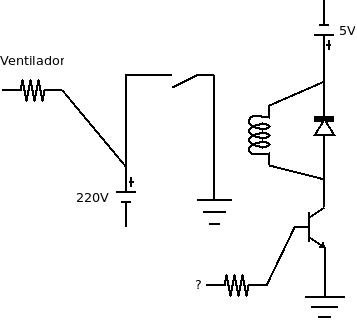
\includegraphics[scale=0.7]{img/breeze-diagram-1.jpg}
    \caption{Circuito (Draft)}
\end{figure}
